\documentclass[border=0pt]{standalone}

\usepackage{enumitem}

\usepackage[sc]{mathpazo}
\usepackage{tikz}
\linespread{1.05}

\newcommand\bluebullet{%
  \tikz[baseline=0ex]\fill[blue!75!black]
    (0,0)--(0.18,0.09)--(0,0.18)--cycle;}


\usepackage[table]{xcolor}
\definecolor{petrol}{RGB}{117,208,98}


\usepackage{tikz}
\usetikzlibrary{calc}


\usepackage{ragged2e}

\begin{document}
\small

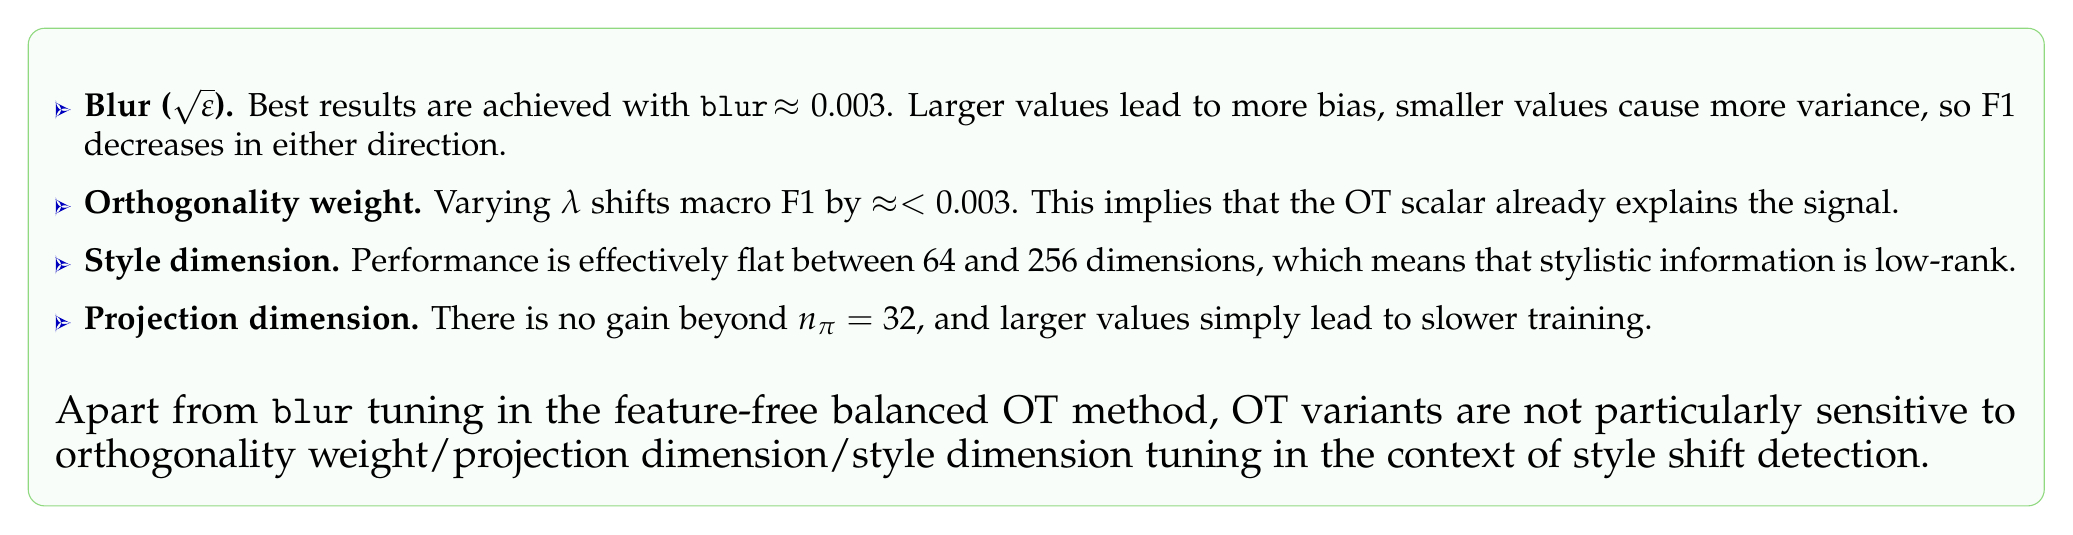
\begin{tikzpicture}
\node[
  draw=petrol!80,              
  fill=petrol!4,              
  rounded corners=6pt,
  minimum width=0.1\linewidth, 
  inner sep=10pt,               
  text width=2.1\linewidth-16pt, 
  font=\large,
  align=justify                
] (cap) {%
\begin{itemize}[label=\bluebullet,left=0em,itemsep=3pt]
\item \textbf{Blur ($\sqrt{\varepsilon}$).} Best results are achieved with $\texttt{blur}\!\approx 0.003$. Larger values lead to more bias, smaller values cause more variance, so F1 decreases in either direction.
  \item \textbf{Orthogonality weight.} Varying \(\lambda\) shifts macro F1 by $\approx<0.003$. This implies that the OT scalar already explains the signal.
  \item \textbf{Style dimension.} Performance is effectively flat between $64$ and $256$ dimensions, which means that stylistic information is low-rank.
  \item \textbf{Projection dimension.} There is no gain beyond \(n_\pi=32\), and larger values simply lead to slower training.
\end{itemize}
\bigskip
\noindent {\Large Apart from \texttt{blur} tuning in the feature-free balanced OT method, OT variants are not particularly sensitive to orthogonality weight/projection dimension/style dimension tuning in the context of style shift detection.}
};
\end{tikzpicture}

\end{document}